\anhang{AWS Well Architected Referenzarchitekturen}
Folgend sind die Referenzarchitekturen aus dem \ac{AWS} Well Architected Framework - Analyticss Lens abgebildet.
\begin{figure}[H]
\centering
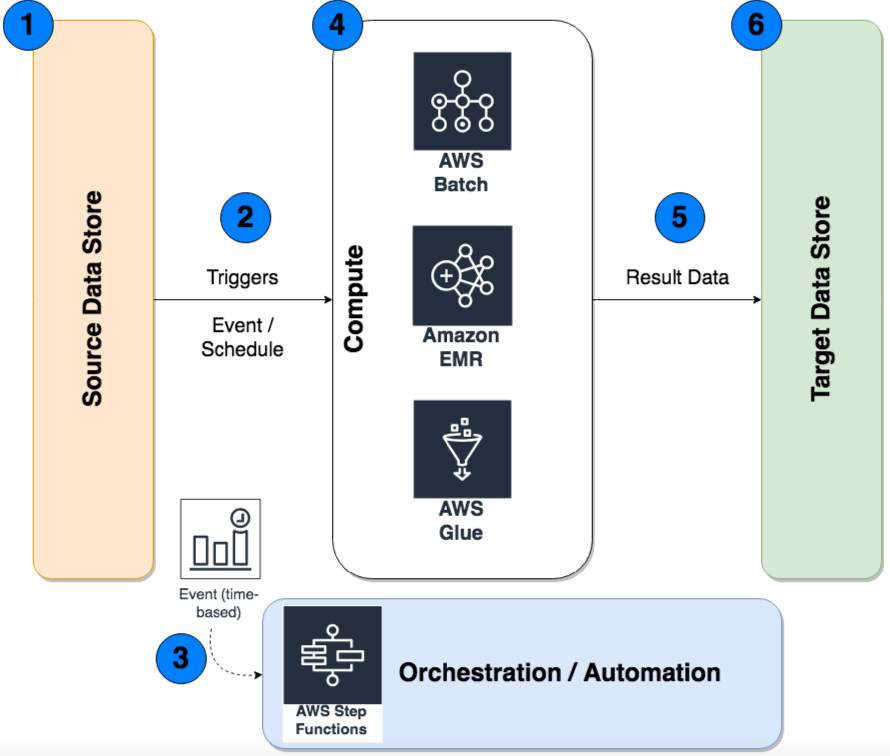
\includegraphics[width=\textwidth]{graphics/AWS-Batch-Architecture.pdf}
\caption[AWS Well Architected Batch Architektur]{AWS Well Architected Batch Architektur.\footnotemark}
\label{abb:AWSWellArchitectedBatch}
\end{figure}
\footnotetext{Entnommen aus: \cite[][12]{Ravirala.2020}}

\begin{figure}[H]
\centering
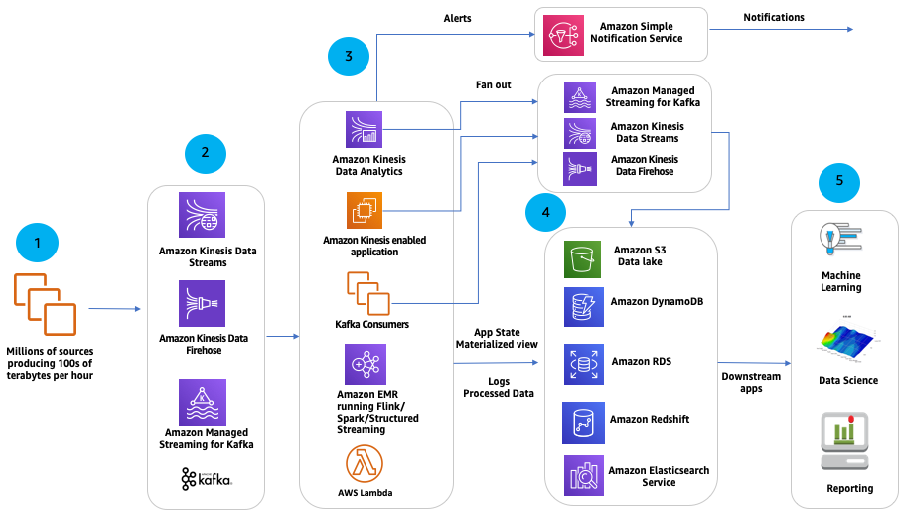
\includegraphics[width=0.92\textheight,angle=90,origin=c]{graphics/AWS-Stream-Architecture.pdf}
\caption[AWS Well Architected Stream/$\kappa$ Architektur]{AWS Well Architected Stream/$\kappa$ Architektur.\footnotemark}
\label{abb:AWSWellArchitectedStream}
\end{figure}
\footnotetext{Entnommen aus: \cite[][15]{Ravirala.2020}}

\begin{figure}[H]
\centering
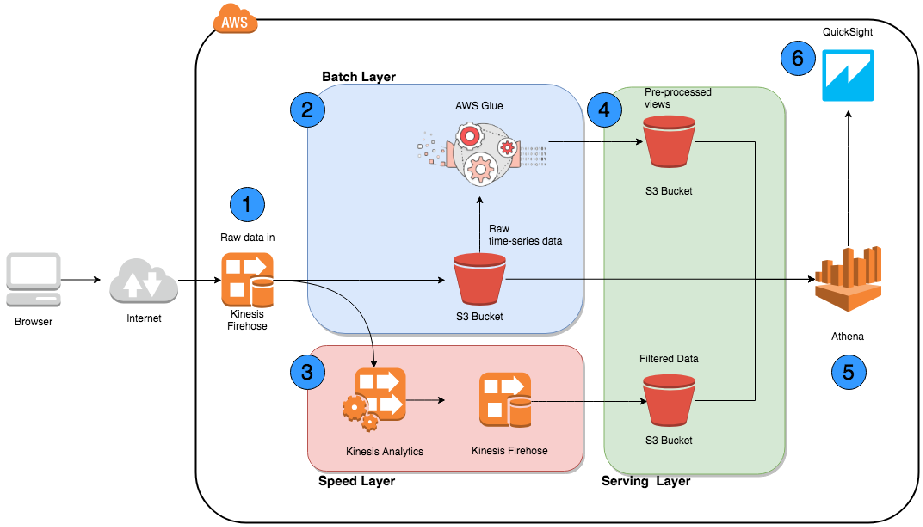
\includegraphics[width=0.92\textheight,angle=90,origin=c]{graphics/AWS-Lambda-Architecture.pdf}
\caption[AWS Well Architected $\lambda$ Architektur]{AWS Well Architected $\lambda$ Architektur.\footnotemark}
\label{abb:AWSWellArchitectedLambda}
\end{figure}
\footnotetext{Entnommen aus: \cite[][18]{Ravirala.2020}}